\section{Databasedesign}
\myworries{Lav noget alla det her \url{https://i.stack.imgur.com/CT1s3.png}}

Denne sektion skal indeholde:

\begin{itemize}
    \item Overvejelser, beslutninger og resultater vedr. tabeldesign og SQL-forespørgsler\\ 
\end{itemize}

\noindent
Denne sektion har til formål at fremvise overvejelserne, beslutningerne og resultaterne vedrørende tabeldesign og SQL-forespørgelser.\\

\subsection{Overvejelser \& beslutninger}
Det første gruppen gjorde var, at finde ud af hvad der skulle opbevares i databasen. 


\subsection{Resultater}
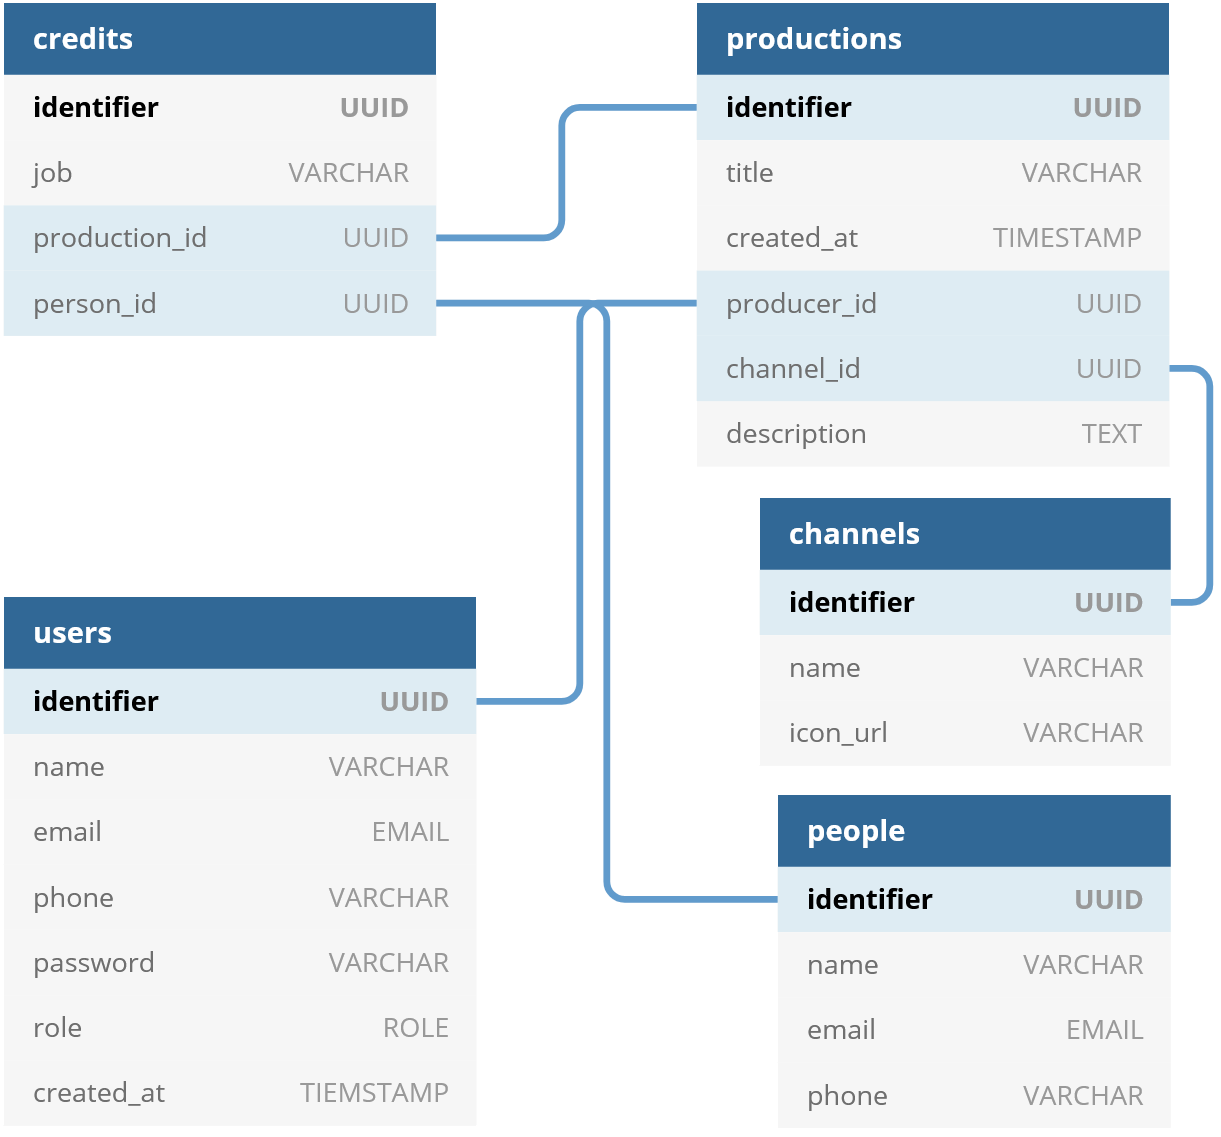
\includegraphics[scale=0.35]{figures/database_design.PNG}
% channels

% ------ code snippet --------
\noindent
CREATE TABLE\\
(\\
identifier UUID NOT NULL,\\
name VARCHAR(512) NOT NULL,\\
PRIMARY KEY (identifier)\\
);\\

\begin{table}[ht]
    \begin{tabularx}{\textwidth}{|X|X|}
        \hline
        \textbf{identifer} &  \textbf{name}\\
        \hline
        a4226ce8-e973-4de3-906b-ac4a696c7cdb & TV2 \\
        \hline
    \end{tabularx}
    \caption{Tabeldesign: channels}
    \label{tab:channel_table}
\end{table}



%\noindent
%CREATE INDEX channels_name_idx ON channels USING btree (name);\\

% productions
\begin{table}[ht]
    \begin{tabularx}{\textwidth}{|X|X|X|X|X|}
        \hline
        \textbf{identifer} &  \textbf{title} & \textbf{created\_at} & \textbf{producer\_id} & \textbf{channel\_id}\\
        \hline
        58cb7c91-ed0a-4bd3-80b8-606690441293 & Stuff & 2008-11-11 & 2f477718-3351-4d97-95dd-12518675ed52 &  a4226ce8-e973-4de3-906b-ac4a696c7cdb\\
        \hline
    \end{tabularx}
    \caption{Tabeldesign: productions}
    \label{tab:productions_table}
\end{table}

% ------ code snippet --------

% users
\begin{table}[ht]
    \begin{tabularx}{\textwidth}{|X|X|X|X|X|}
        \hline
        \textbf{identifer} &  \textbf{name} & \textbf{email} & \textbf{password} & \textbf{role}\\
        \hline
        2f477718-3351-4d97-95dd-12518675ed52 & Simon & string@string.dk &  string & 3\\
        \hline
    \end{tabularx}
    \caption{Tabeldesign: users}
    \label{tab:users_table}
\end{table}

% ------ code snippet --------

